\documentclass[10pt,a4paper,twocolumn]{article}
\usepackage{commands}


\usepackage{natbib} 
%\setcitestyle{authoryear, open={([},close={)]}}
%\setcitestyle{numbers,square}
\bibliographystyle{dinat}

\title{On the Laplacian}
\author{Ali Fele-Paranj}

\begin{document}
	\maketitle
	\begin{abstract}
		I have gathered the sporadic contents on the notion of Laplacian in different settings (like defined for graphs, infinite graphs, real space ($ \R $) as well as on the manifolds).
	\end{abstract}
	\section{Laplacian Matrix of a Graph}
	For a graph, the Laplacian matrix contains the information on the in/out flow of stuff into the nodes.
	\begin{figure}[h!]
		\centering
		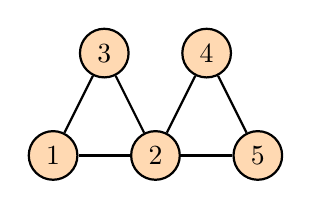
\begin{tikzpicture}[scale=1.3, auto, every node/.style={circle, draw=black, fill=orange!30, thick, minimum size=5mm}]
			% Nodes
			\node (n1) at (0,0) {1};
			\node (n2) at (1,0) {2};
			\node (n3) at (0.5,1) {3};
			\node (n4) at (1.5,1) {4};
			\node (n5) at (2,0) {5};
			
			% Edges (randomly chosen but ensuring connectivity)
			\draw[thick] (n1) -- (n3);
			\draw[thick] (n1) -- (n2);
			\draw[thick] (n3) -- (n2);
			\draw[thick] (n4) -- (n2);
			\draw[thick] (n4) -- (n5);
			\draw[thick] (n2) -- (n5);
		\end{tikzpicture}
	\end{figure}
	Then the Laplacian matrix is given by
	\[ D = \begin{pmatrix}
		2 & 0 & 0 & 0 & 0 \\
		0 & 4 & 0 & 0 & 0 \\
		0 & 0 & 2 & 0 & 0 \\
		0 & 0 & 0 & 2 & 0 \\
		0 & 0 & 0 & 0 & 2
	\end{pmatrix}, \]
	and the adjacency matrix  is given by
	\[ A = \begin{pmatrix}
		0 & 1 & 1 & 0 & 0 \\
		1 & 0 & 1 & 1 & 1 \\
		1 & 1 & 0 & 0 & 0 \\
		0 & 1 & 0 & 0 & 1 \\
		0 & 1 & 0 & 1 & 0
	\end{pmatrix}, \]
	and the Laplacian matrix is given by
	\[ L = D -A = 
	 \begin{pmatrix}
		2 & -1 & -1 & 0 & 0 \\
		-1 & 4 & -1 & -1 & -1 \\
		-1 & -1 & 2 & 0 & 0 \\
		0 & -1 & 0 & 4 & -1 \\
		0 & -1 & 0 & -1 & 5
	\end{pmatrix}.
	 \]
	It is straight forward to generalize the notion of Laplacian matrix to the weighed graphs, where the degree matrix $ D $, the diagonal entries will be the sum of all weights of the edges connected to that node, and for the adjacency matrix, instead of zeros and ones, we will have the weights of the connections..
	
	There is also another way of finding the Laplacian matrix by using the notion of incidence matrix. To do so, we first need to make our graph to be directed. Any combination of the direction on the edges will do the job and will yield in a correct answer. For instance, consider the following directed graph
	
	\begin{figure}[h!]
		\centering
		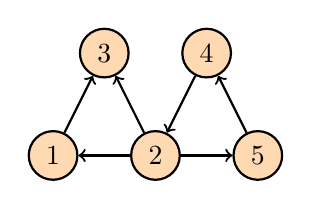
\begin{tikzpicture}[scale=1.3, auto, every node/.style={circle, draw=black, fill=orange!30, thick, minimum size=5mm}]
			% Nodes
			\node (n1) at (0,0) {1};
			\node (n2) at (1,0) {2};
			\node (n3) at (0.5,1) {3};
			\node (n4) at (1.5,1) {4};
			\node (n5) at (2,0) {5};
			
			% Edges (randomly chosen but ensuring connectivity)
			\draw[->,thick] (n1) -- (n3);
			\draw[<-,thick] (n1) -- (n2);
			\draw[<-,thick] (n3) -- (n2);
			\draw[->,thick] (n4) -- (n2);
			\draw[<-,thick] (n4) -- (n5);
			\draw[->,thick] (n2) -- (n5);
		\end{tikzpicture}
	\end{figure}
	
	Its incidence matrix will be
	\[
	M = \begin{pmatrix}
		-1 & 1  & 0  & 0  & 0  & 0  \\
		0  & -1 & 1  & -1 & 0  & -1 \\
		1  & 0  & -1 & 0  & 0  & 0  \\
		0  & 0  & 0  & 1  & 1  & 0  \\
		0  & 0  & 0  & 0  & -1 & 1  \\
	\end{pmatrix}
	\]
	The Laplacian matrix can be written as
	\[ \mathcal{L} = M M^T. \]
	Note that in the case of the weighed graphs, we will have
	\[ \mathcal{L} = M W M^T \tag{1}\]
	where $ W $ is a diagonal matrix containing the weights. These computations can be done easily on the NetworkX. 
	
	\begin{minted}[tabsize=2,breaklines,fontfamily=courier]{python}
	g = nx.Graph()
	for i in range(1,6):
		g.add_node(i)
		
		g.add_edge(1,2,w=1)
		g.add_edge(1,3,w=2)
		g.add_edge(2,3,w=3)
		g.add_edge(2,5,w=5)
		g.add_edge(4,5,w=5)
	
	W = np.diag([data['w'] for u, v, data in g.edges(data=True)])
	
	% adj matrix
	AD = nx.adjacency_matrix(g,weight="w")
	
	% Laplacian matrix
	L = nx.laplacian_matrix(g,weight="w")
	
	% Incidence matrix
	inc_matrix = nx.incidence_matrix(g,oriented=True)
	\end{minted}
	
	
	The incidence matrix is also very useful in calculating the pressure difference between nodes of a particular edge. Let $ \Delta = M^T $. Then given the vector $ P $ that contains the pressures on the vertices, then the pressure difference on the edges will be given by $ \Delta P $, where $ \Delta  $ is the transpose of the incidence matrix. This comes in handy when we want to calculate the flow of the edges which will be given by
	 \[ \bf{Q} = \bf{C} L^{-1} \bf{\Delta} \bf{P}, \tag{2} \]
	where $ C $ is a diagonal matrix of the conductance of the edges, $ L $ is the diagonal matrix of the ``length'' of each edge, $ \Delta $ is the transpose of the incidence matrix, and $ P $ is the pressure on the nodes. $ Q $ is the flow of the edges. In this particular example we are assuming that the relation between flow and the pressure difference is $ Q_e = C_e (p_i - p_j)/L $. But we can have many other choices.
	
	Knowing the sources and sinks on the nodes, the pressure can be determined by the Kirchhoff law
	\[ \mathcal{L} \bf{P} = \bf{q}, \]
	where the vector $ q $ is the sources and the sinks values for each node. This is the same as solving the \textbf{Poisson equation}. This can also be written in terms of the flow, i.e.
	\[ \Delta^T \bf{Q} = \bf{q}. \] 
	By $ (2) $ we can write
	\[ (\bf{\Delta}^T \bf{C}\bf{L}^{-1}\Delta) \bf{P} = \bf{q}. \]
	Since $ \Delta = M^T $, the expression inside the parentheses is clearly Equation (1).
	
	Similar to the Poisson equation on the graph which is equivalent Kirchhoff's law, we can solve other types of heat and wave equations on the graph as well. The Laplacian matrix play a key role.
	\[ \frac{\partial p}{\partial t} = - \mathcal{L} p + q,  \] 
	for the heat equation, and
	\[ \frac{\partial^2 p}{\partial t^2} = -\mathcal{L}p + q, \]
	for the wave equation.
	
	\section{Laplacian Operator of Infinite Graphs}
	In analogy with the Laplacian matrix for the graphs, we can develop a similar notion for the infinite graphs, in particular infinite Cayley graphs. In short, given a group $ G $ and a generating set $ S $ (where $ S $ is a subset of $ G $ not containing the identity and closed under taking inverses if the graph is to be undirected), the Cayley graph $ \Gamma(G,S) $ is defined as follows
	\begin{itemize}
		\item Vertices: Each element of $ G $ corresponds to a vertex.
		\item Edges: There is an edge between $ g $ and $ gs $ fo every $ g\in G $ and $ s \in S $.
	\end{itemize}
	In the case of the infinite graphs, we can not define an infinite dimensional Laplacian matrix, but instead we can define an operator. For an infinite Cayley graph $ \Gamma(G,S) $, the \textbf{Laplacian} that acts on a function $ f: G \to C $ (note that the set of vertices is the group it self) can be defined as
	\[ (\Delta f)(g) = \sum_{s\in S} (f(g) - f(gs)) = |S|f(g) - \sum_{s\in S} f(gs). \]
	There is a close parallel between the definition above and the definition of the Laplacian matrix of a graph $ \mathcal{L} = D - A $. For instance, in the case of a Cayley graph of $ \Z^2 $ we have
	\[ (\Delta f)(i,j) = 4 f(i,j) - f(i+1,j) - f(i-1,j) - f(i,j+1) - f(i,j-1). \]
	This coincides with the notion of the discrete finite difference Laplacian operator.
	
%	
%	\newpage
%	\bibliography{References/references}
\end{document}